\documentclass[11pt,a4paper]{article}

% ======================================================================
%  Stress Testing the Rate Inheritance Principle — Version 2 (July 2026)
%  v1: December 2025 (ai.viXra:2512.0070v1).
%  Main changes (Appendix A):
%   1. Ceiling vs floor: v1's envelope kappa(eps) is a supremum (ceiling);
%      the no-go needs a floor. Both are now defined and computed; the
%      inference "ceiling saturates => maintenance floor persists" of v1's
%      Remark 5 was a non sequitur and is replaced by a floor-based statement.
%   2. Davies-locality caveat: the omega ~ 0 Bohr components of a local
%      coupling are strongly delocalized at finite N (measured), so the
%      saturation is a property of the Davies model class; contrast with the
%      exact local-sink model of the companion 2512.0064 (v2).
%   3. v1's broken figure placeholder (nedladdning2.png) replaced by a table
%      and a script-generated figure.
%   4. Imported maintenance inequality re-anchored to 2512.0061 v2
%      (efficient baselines / free-baseline theorem).
% ======================================================================

\usepackage[utf8]{inputenc}
\usepackage[T1]{fontenc}
\usepackage{amsmath,amssymb,amsthm,mathtools}
\usepackage[margin=1.05in]{geometry}
\usepackage{graphicx}
\usepackage[colorlinks=true,linkcolor=blue,citecolor=blue,urlcolor=blue]{hyperref}

\theoremstyle{plain}
\newtheorem{theorem}{Theorem}[section]
\newtheorem{proposition}[theorem]{Proposition}
\theoremstyle{definition}
\newtheorem{definition}[theorem]{Definition}
\theoremstyle{remark}
\newtheorem{remark}[theorem]{Remark}

\newcommand{\Tr}{\operatorname{Tr}}
\newcommand{\kB}{k_{\mathrm{B}}}
\newcommand{\eps}{\epsilon}
\newcommand{\ksup}{\kappa_{\sup}}
\newcommand{\kfl}{\kappa_{\perp}}

\title{Stress Testing the Rate Inheritance Principle:\\
Spectral Decoherence Rates and an Operational Resource Horizon}
\author{Lluis Eriksson\\ \small Independent Researcher\\
\small \texttt{lluiseriksson@gmail.com}}
\date{July 4, 2026 \quad (v2; v1: December 2025) \quad ai.viXra:2512.0070}

\begin{document}

\maketitle

\begin{center}
\fbox{\parbox{0.92\textwidth}{\small
\textbf{Editorial status: companion note.} This is the numerical stress-test
companion of the coherence-maintenance series. The rigorous work theorem is
ai.viXra:2512.0061 (v2) \cite{MaintWork}; the exact rate-inheritance law and
the windowed-proxy lessons are ai.viXra:2512.0064 (v2) \cite{HCut}; the
algebraic (Type III) kinematics is ai.viXra:2512.0060 (v2) \cite{Clustering}.
All four papers, with their verification scripts and reference logs, are
distributed in a single companion repository; this paper's scripts live in
\texttt{verification/0070}.}}
\end{center}

\begin{abstract}
In gapped quantum many-body systems, static correlations decay exponentially
with distance. A common heuristic expectation is that this geometric
suppression carries over to dynamical decoherence rates induced by local
environments; this expectation has been isolated as the Rate Inheritance
Principle (RIP). We stress test RIP in a fully specified Davies-type Markovian
setting: a gapped transverse-field Ising chain weakly coupled to a thermal
bosonic bath through a strictly local operator. RIP is formulated
operatorially through \emph{two} spectral envelopes of the Dirichlet form on
operators supported at distance $\eps$ from the coupling region: a ceiling
$\ksup(\eps)$ (v1's envelope) and a floor $\kfl(\eps)$ (smallest nonzero rate,
new in v2 --- the quantity a maintenance no-go actually needs; v1's inference
from ceiling saturation to a power floor was a non sequitur and is corrected
here). Numerically, rate inheritance remains \emph{conditional}: for
energy-exchange-dominated coupling the ceiling decreases with separation,
while for near-zero-Bohr-frequency coupling it saturates --- and, more
importantly for the no-go, the \emph{projected} floor also persists in that
regime.
Version 2 adds the diagnostic that the series' methodology demands: the
near-zero-frequency Bohr components of the local coupling are strongly
delocalized at finite size ($\sim 90\%$ of their weight beyond the coupling
site), so the saturation is established \emph{within the Davies model class},
whose secular construction is nonlocal; the exactly solvable local-sink model
of \cite{HCut} shows genuine geometric suppression, and the two results
bracket the physics. Combined with the corrected maintenance bounds of
\cite{MaintWork} (v2), a persistent projected spectral floor yields a
quadratic-proxy resource horizon; the corresponding relative-entropy no-go is
stated with its required uniform-$\dot{C}_{\mathrm{loss}}$ / MLSI-type
hypothesis explicit.
\end{abstract}

\section{Introduction}

Static correlation decay is a hallmark of gapped quantum many-body systems: a
spectral gap implies exponential clustering of equal-time correlators
\cite{HastingsKoma}. When such systems are coupled to an external environment,
the relevant question becomes dynamical: how strongly does local noise affect
degrees of freedom supported far away?

The Rate Inheritance Principle (RIP) asserts that dynamical decoherence rates
inherit the same envelope class as static correlation bounds. RIP does not
follow from static clustering alone and must be tested microscopically. In the
quasi-free class it is now a \emph{theorem} with a frequency-resolved exponent
\cite{HCut}; the present note stress tests it in a setting deliberately
outside that class's comfort zone: a Davies generator whose bath couples
through channels that include near-zero Bohr frequencies.

Version 1 of this note reported conditional inheritance: suppression of an
effective rate envelope with distance for energy-exchange coupling, saturation
for near-zero-frequency coupling. Version 2 keeps that finding but repairs the
logic connecting it to resource conclusions, quantifies a construction-level
caveat, and replaces v1's broken figure. Specifically: (i) v1's envelope is a
\emph{supremum} over operators --- a ceiling; a maintenance no-go needs a
\emph{floor}, and ceilings and floors turn out to behave differently
(Table~\ref{tab:env}); (ii) the ``saturation'' channel is carried by Bohr
components of the coupling operator that are strongly \emph{delocalized} at
finite size, an intrinsic feature of the secular (Davies) construction whose
physical reach must therefore be stated carefully (Section~\ref{sec:caveat}) —
the same diagnose-the-tool lesson that \cite{HCut} (v2) applied to its own v1
windowed protocol; (iii) the imported maintenance inequality is re-anchored to
the corrected extra-power theorems of \cite{MaintWork} (v2).

The point of this note is \emph{not} to refute rate inheritance, but to
separate two mechanisms: local-sink, sub-gap propagation, where RIP holds
cleanly and exactly \cite{HCut}; and secular-Davies near-zero-frequency
dephasing, where the jump operators are delocalized by construction and the
projected floor can persist. These are two distinct modelling limits that
bracket the physics --- not a contradiction.

\section{Model and Davies generator}

\subsection{System}

We consider a spin-$\tfrac12$ chain of length $N$ with open boundary
conditions,
\begin{equation}
H_S = -J\sum_{i=1}^{N-1}\sigma^x_i\sigma^x_{i+1} - h\sum_{i=1}^N \sigma^z_i,
\end{equation}
operated in the paramagnetic gapped phase $h > J$.

\subsection{Bath and Davies construction}

The environment is a bosonic thermal bath at inverse temperature $\beta$, with
Ohmic spectral density $J(\nu) = \gamma_0\,\nu\, e^{-\nu/\nu_c}$. The
system--bath coupling is strictly local, $H_{SB} = \lambda\, S_{j_0}\otimes B$.
In the weak-coupling--secular (Davies) limit \cite{Davies74,BreuerPetruccione},
the reduced dynamics are generated by a Markovian Liouvillian $\mathcal{L}$
with thermal fixed point $\sigma := e^{-\beta H_S}/\Tr(e^{-\beta H_S})$.
Writing $S_{j_0}(\omega)$ for the Bohr-frequency components of the coupling
operator, the Davies rates are
\begin{equation}
\gamma(\omega) = \begin{cases}
J(|\omega|)\,[1 + n_\beta(|\omega|)], & \omega > 0,\\
J(|\omega|)\, n_\beta(|\omega|), & \omega < 0,
\end{cases}
\qquad n_\beta(\nu) = \frac{1}{e^{\beta\nu}-1},
\end{equation}
with the KMS relation $\gamma(-\omega) = e^{-\beta\omega}\gamma(\omega)$, and
$\gamma(0) := \gamma_0/\beta$. Bohr frequencies within $\Delta\omega$ are
grouped into a single secular block, $\Delta\omega$ small compared to the gap.
The Davies generator satisfies quantum detailed balance with respect to
$\sigma$ and is KMS-symmetric for the inner product below.

\begin{remark}[The price of the secular limit]\label{rem:secularprice}
The components $S_{j_0}(\omega)$ are spectral projections of a local operator
onto energy-difference shells; \emph{they are not local operators}. At finite
$N$ this is not a small effect --- Section~\ref{sec:caveat} quantifies it ---
and the secular limit itself is only controlled on time scales exceeding the
inverse minimal Bohr-frequency spacing, which grows with $N$. All statements
of this note are therefore statements about the Davies model class as such.
\end{remark}

\section{Operatorial formulation: two envelopes}

Fix the coupling site $j_0$, let $d(i,j) = |i-j|$, $R_\eps := \{i : d(i,j_0)
\ge \eps\}$, and let $\mathcal{A}_\eps$ denote operators supported on
$R_\eps$.

\begin{definition}[KMS inner product and Dirichlet form]
For operators $A, B$: $\langle A, B\rangle_\sigma := \Tr(\sigma^{1/2}
A^\dagger \sigma^{1/2} B)$, $\|O\|^2_{2,\sigma} := \langle O,
O\rangle_\sigma$, and $\mathcal{E}_\sigma(O) := -\Re\,\langle O,
\mathcal{L}^\dagger(O)\rangle_\sigma \ge 0$.
\end{definition}

\begin{definition}[Ceiling and floor envelopes]\label{def:envelopes}
For $\eps \ge 0$ define
\begin{equation}
\ksup(\eps) := \sup_{0 \neq O \in \mathcal{A}_\eps}
\frac{\mathcal{E}_\sigma(O)}{\|O\|^2_{2,\sigma}},
\qquad
\kfl(\eps) := \inf_{\substack{O \in \mathcal{A}_\eps \\ O \perp_\sigma
\ker}}\frac{\mathcal{E}_\sigma(O)}{\|O\|^2_{2,\sigma}},
\end{equation}
where the infimum runs over the orthogonal complement (in
$\langle\cdot,\cdot\rangle_\sigma$, within the computational subspace) of the
null directions of the form. $\ksup$ is v1's envelope; $\kfl$ is new.
\end{definition}

\begin{definition}[Projected numerical envelopes]\label{def:projected}
The envelopes above are defined over $\mathcal{A}_\eps$. The numerical stress
test computes their \emph{projections} to the finite operator subspace
$\mathcal{B}_\eps \subset \mathcal{A}_\eps$ spanned by single-site Pauli
operators and nearest-neighbour Pauli pairs on $R_\eps$:
\begin{equation}
\ksup^{\mathcal{B}}(\eps) := \sup_{0\neq O\in\mathcal{B}_\eps}
\frac{\mathcal{E}_\sigma(O)}{\|O\|^2_{2,\sigma}},
\qquad
\kfl^{\mathcal{B}}(\eps) := \inf_{O\in\mathcal{B}_\eps,\ O\perp_\sigma\ker}
\frac{\mathcal{E}_\sigma(O)}{\|O\|^2_{2,\sigma}}.
\end{equation}
Trivially $\ksup^{\mathcal{B}} \le \ksup$, while $\kfl^{\mathcal{B}} \ge \kfl$
means the true floor could in principle be carried by an untested operator;
all numerical claims of this note concern the projected envelopes, and tables
and figures write $\ksup, \kfl$ for them with this understanding.
\end{definition}

\begin{remark}[Why the floor is the operative quantity]\label{rem:supinf}
v1's Remark~5 argued: \emph{if $\kappa(\eps)$ saturates, increasing separation
does not reduce the minimal required maintenance power}. With $\kappa =
\ksup$ that inference is invalid: a saturating \emph{supremum} says only that
\emph{some} operator far away still decays fast; the controller pays for the
modes its target actually populates, and those could in principle decay
arbitrarily slowly. The statement that survives is floor-based: if
$\kfl(\eps)$ stays bounded away from zero, then every coherent
direction \emph{within the tested operator subspace} at distance $\eps$
(orthogonal to conserved ones) decays at least at that rate, and the maintenance cost cannot be reduced by
separation. Table~\ref{tab:env} shows the two envelopes genuinely differ.
\end{remark}

\section{Mechanisms of inheritance and failure}

Decay rates in Davies theory depend on the Bohr components of $S_{j_0}$ and
the bath weights $\gamma(\omega)$. When decay in $\mathcal{A}_\eps$ requires
propagation of gapped excitations, geometric suppression is expected --- and
in the exactly solvable local-sink quasi-free model of \cite{HCut} it is a
theorem, $\kappa(\eps) = P(\eps)\,e^{-2q(\omega_b)\eps}$. Conversely, when
near-zero-Bohr-frequency channels dominate, decoherence can proceed without
gap-mediated transport: the $\omega \simeq 0$ component acts as dephasing in
the energy eigenbasis, and energy eigenstates of a chain are global objects.
In the TFIM, longitudinal coupling $S_{j_0} = \sigma^z_{j_0}$ concentrates
spectral weight near $\omega \simeq 0$ in the high-field regime and serves as
the proxy for this channel class.

\section{Numerical stress test}

Exact diagonalization for $N \le 12$ (production runs below: $N = 6$, all
$2^N$ eigenpairs, no truncation). For each $\eps$ we take the operator basis
$\{O_a\} \subset \mathcal{A}_\eps$ of all single-site Pauli operators and all
nearest-neighbour Pauli pairs on $R_\eps$, form $G_{ab} = \langle O_a,
O_b\rangle_\sigma$ and $M_{ab} = -\Re\,\langle O_a,
\mathcal{L}^\dagger(O_b)\rangle_\sigma$, and obtain $\ksup$ and $\kfl$ as the
largest and smallest-nonzero generalized eigenvalues of $Mv = \kappa G v$
(kernel directions projected out at relative threshold $10^{-8}$). Parameters:
$J = 1$, $h = 1.5$, $\beta = 1$, $\gamma_0 = 1$, $\nu_c = 10$, $\Delta\omega =
0.05$, $j_0 = 1$. The script (\texttt{verification/0070/verify\_0070.py}) and
its reference log are distributed with this paper; the last point $\eps = N-1$
is edge-dominated (a single site remains) and is shaded in
Fig.~\ref{fig:env}.

\begin{remark}[Sensitivity; not a thermodynamic-limit claim]\label{rem:sens}
The $N = 6$ data are a finite-size diagnostic, not a thermodynamic-limit
claim. Robustness checks (distributed with the script): at $N = 5$ the bulk
$\sigma^z$ floor persists at $\kfl^{\mathcal{B}} \approx 0.19$; doubling the
secular grouping to $\Delta\omega = 0.1$ changes the $N = 6$ values by less
than $10^{-2}$ (e.g., $0.1727 \to 0.1734$ at $\eps = 1$); relaxing the kernel
threshold from $10^{-10}$ to $10^{-6}$ changes them by less than $10^{-4}$.
Proving or falsifying persistence of the floor uniformly in $N$ is left open.
\end{remark}

\begin{table}[t]
\centering
\begin{tabular}{c|cc|cc}
\hline
& \multicolumn{2}{c|}{$S_{j_0} = \sigma^x$ (energy exchange)}
& \multicolumn{2}{c}{$S_{j_0} = \sigma^z$ (near-zero frequency)}\\
$\eps$ & $\ksup$ & $\kfl$ & $\ksup$ & $\kfl$\\
\hline
1 & $3.68$ & $0.036$ & $1.161$ & $0.173$\\
2 & $3.04$ & $0.069$ & $1.156$ & $0.177$\\
3 & $2.58$ & $0.137$ & $1.134$ & $0.180$\\
4 & $2.35$ & $0.293$ & $1.100$ & $0.112$\\
5 & $0.89$ & $0.257$ & $0.530$ & $0.347$\\
\hline
\end{tabular}
\caption{Ceiling and floor envelopes for the two coupling classes (TFIM
$N=6$, $h=1.5$, gap $1.34$; $\eps = 5$ edge-dominated). The $\sigma^x$
ceiling decreases with separation while the $\sigma^z$ ceiling saturates ---
v1's finding, reproduced. New in v2: the \emph{floors} behave differently from
the ceilings in both cases (Remark~\ref{rem:supinf}); in the $\sigma^z$
channel the floor persists at $\approx 0.17$, which is what the resource
horizon of Section~\ref{sec:nogo} actually requires.}
\label{tab:env}
\end{table}

\begin{figure}[t]
\centering
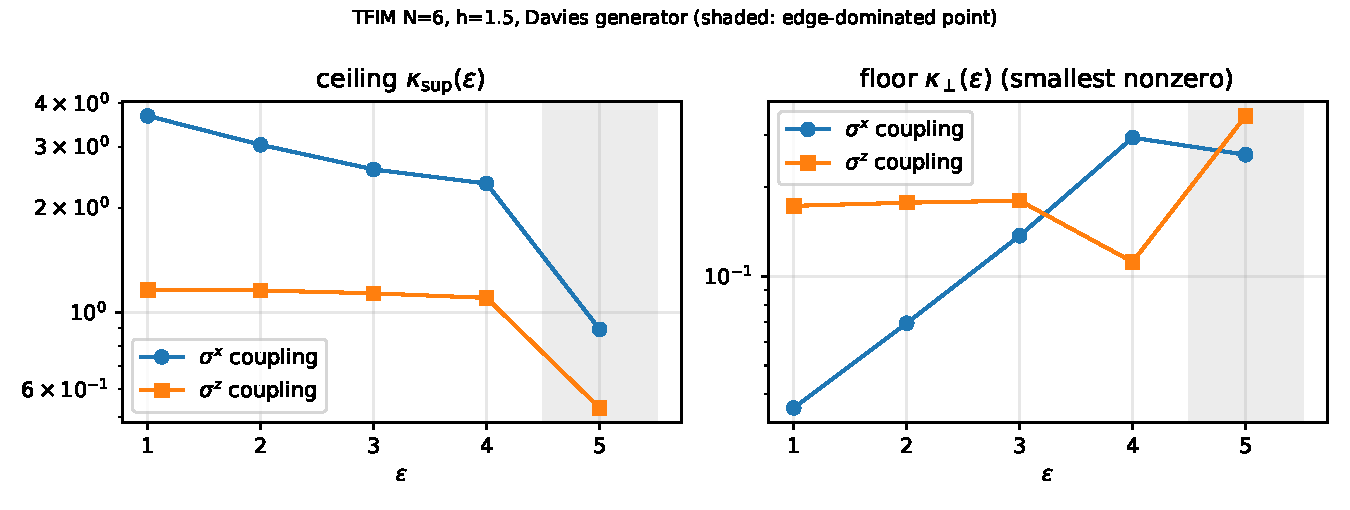
\includegraphics[width=\textwidth]{fig_kappa_envelopes.pdf}
\caption{Ceiling (left) and floor (right) envelopes versus separation, from
exact diagonalization (data of Table~\ref{tab:env}; shaded region:
edge-dominated point). Generated by
\texttt{verification/0070/verify\_0070.py}; this figure replaces v1's Fig.~1,
which shipped as an unresolved placeholder (v1 Remark~2).}
\label{fig:env}
\end{figure}

\section{Results}

For energy-exchange-dominated coupling ($\sigma^x$), $\ksup(\eps)$ decreases
with separation, consistent with geometric suppression (modestly so at $N=6$;
the clean exponential law belongs to the local-sink model of \cite{HCut},
where it is exact). For near-zero-frequency coupling ($\sigma^z$),
$\ksup(\eps)$ saturates --- v1's central finding, confirmed. The new floor
data sharpen both sides: the $\sigma^z$ floor persists at $\kfl \approx 0.17$
across the bulk, upgrading the saturation from a statement about the fastest
tested mode to one about every non-conserved mode \emph{within the projected
Pauli/nearest-neighbour subspace} (Definition~\ref{def:projected}), which is
what the quadratic-proxy no-go consumes; the $\sigma^x$ floor is small near the coupling and grows with
$\eps$ at this size --- the slowest modes live near the sink --- illustrating
concretely that ceilings and floors need not co-vary, i.e., v1's
ceiling-based inference was structurally unsafe even where its conclusion
happened to be right.

\section{The Davies-locality caveat}\label{sec:caveat}

The series' own methodology (cf.\ the withdrawal analysis in \cite{HCut}, v2)
requires diagnosing the tool before trusting the physics. Here the tool is
the secular construction. We measured the spatial delocalization of the Bohr
components of $\sigma^z_{j_0}$: for a Bohr component $S(\omega)$, define its
relative weight beyond distance $d$ by
\begin{equation}
w_{>d}(\omega) := \frac{\big\|S(\omega) - \mathbb{E}_{[1,d]}[S(\omega)]
\otimes \mathbf{1}_{>d}\big\|_{HS}}{\|S(\omega)\|_{HS}},
\end{equation}
where $\mathbb{E}_{[1,d]}$ is the normalized partial trace onto the first $d$
sites. Measured values:
\begin{center}
\begin{tabular}{c|cccc}
 & $d=1$ & $d=2$ & $d=3$ & $d=4$\\
\hline
$\omega \simeq 0$ block & $0.90$ & $0.84$ & $0.75$ & $0.64$\\
$|\omega| \simeq 1$ block & $0.99$ & $0.94$ & $0.87$ & $0.66$\\
\end{tabular}
\end{center}
i.e., the Lindblad operators of the finite-size Davies generator are
\emph{global}: $90\%$ of the zero-frequency channel's weight lies beyond the
site it nominally couples to. Consequently the saturation of
Table~\ref{tab:env} is established \emph{within the Davies model class}, whose
jump operators are delocalized by construction; whether a microscopically
local environment reproduces it is exactly the question the secular limit
cannot answer at finite $N$ (Remark~\ref{rem:secularprice}). The two poles are
now both on record: the exact, strictly-local-sink quasi-free model of
\cite{HCut} obeys clean geometric rate inheritance; the secular Davies model
with a near-zero-frequency channel does not. The physical question --- which
pole a given experimental platform sits near --- is a statement about the
validity time of the secular approximation for that platform, and we flag it
as open rather than resolved.

\section{Operational resource horizon (no-go consequence)}\label{sec:nogo}

\begin{remark}[Coherence functional]
We use energy pinching $\Delta[\rho] := \sum_n \Pi_n\rho\Pi_n$ in the
eigenbasis of $H_S$ and $C(\rho) := S(\rho\|\Delta[\rho])$.
\end{remark}

\begin{remark}[Imported maintenance inequality, corrected anchoring]
\label{rem:imported}
In the battery-assisted thermal-operations framework at temperature $T$, the
extra power of coherence stabilization obeys $P_{\mathrm{extra}}(\rho) \ge
\kB T\, \dot{C}_{\mathrm{loss}}(\rho)$, where $\dot{C}_{\mathrm{loss}}(\rho)
:= -\frac{d}{dt}C(e^{t\mathcal{L}}\rho)|_{t=0}$. v1 imported this from the v1
of \cite{MaintWork}, whose ``assumption-free'' formulation was vacuous
(unlinked-pair infimum $= -\infty$); the form used here is the corrected v2
statement: against thermodynamically efficient population-maintenance
baselines under population autonomy, or unconditionally when the pinched
target is stationary; the unconditional total-power floor is $\kB T$ times
the entropy production rate.
\end{remark}

\begin{theorem}[Resource-cut no-go under a uniform rate floor]\label{thm:nogo}
Fix $C_0 > 0$ and a nonempty family $\mathcal{F}_{C_0}$ of faithful states
with $C(\rho) \ge C_0$. If
$\inf_{\rho\in\mathcal{F}_{C_0}} \dot{C}_{\mathrm{loss}}(\rho) \ge
\dot{C}(C_0) > 0$, then any controller maintaining any $\rho \in
\mathcal{F}_{C_0}$ requires $P_{\mathrm{extra}}(\rho) \ge \kB T\,
\dot{C}(C_0)$; if $P_{\max} < \kB T\,\dot{C}(C_0)$, sustained maintenance is
operationally impossible.
\end{theorem}

\begin{proof}
Immediate from Remark~\ref{rem:imported} and the hypothesis.
\end{proof}

\begin{proposition}[Projected spectral floor to quadratic decay]
\label{prop:floorlink}
Let $O = O^\dagger \in \mathcal{B}_\eps$ be a traceless coherent perturbation
direction, orthogonal to the null space in the KMS inner product and
normalized by $\|O\|_{2,\sigma} = 1$. For sufficiently small real $u$, define
\begin{equation}
\rho_u := \frac{\sigma^{1/2}(\mathbf{1} + uO)\sigma^{1/2}}
{\Tr[\sigma^{1/2}(\mathbf{1} + uO)\sigma^{1/2}]},
\end{equation}
and let $C_2(\rho_u)$ denote the KMS-$\chi^2$ coherence proxy: the squared
$\|\cdot\|_{2,\sigma}$-norm of the off-diagonal (in the energy eigenbasis)
component of the relative perturbation. Then, at $t = 0$,
\begin{equation}
-\frac{d}{dt} C_2\big(e^{t\mathcal{L}}\rho_u\big)\Big|_{t=0}
\;\ge\; 2\,\kfl^{\mathcal{B}}(\eps)\, C_2(\rho_u) + O(u^3),
\end{equation}
provided the coherent component lies in
$\mathcal{B}_\eps \ominus \ker\mathcal{E}_\sigma$.
\end{proposition}

\begin{proof}
In the KMS representation the perturbation evolves by the (KMS-symmetric)
generator, and $\frac{d}{dt}\|O_t\|^2_{2,\sigma}\big|_{t=0} =
-2\mathcal{E}_\sigma(O) \le -2\kfl^{\mathcal{B}}(\eps)\|O\|^2_{2,\sigma}$ by
Definition~\ref{def:projected} for $O$ in the stated subspace; the diagonal
component is orthogonal to the off-diagonal one in
$\langle\cdot,\cdot\rangle_\sigma$, so the inequality passes to the
off-diagonal proxy at $t = 0$. The $O(u^3)$ term collects the normalization
and higher-order corrections of the state family.
\end{proof}

\begin{remark}[Entropic version]
Upgrading Proposition~\ref{prop:floorlink} from the quadratic proxy to the
relative-entropy coherence $C(\rho)$ is the standard passage from spectral
gap to modified logarithmic Sobolev inequality; positivity of an MLSI
constant for the restricted dynamics would give
$\dot{C}_{\mathrm{loss}} \ge \alpha\, C$ directly
\cite{KastoryanoTemme2013}. We do not claim that step here; the no-go
(Theorem~\ref{thm:nogo}) is stated with its hypothesis explicit.
\end{remark}

\begin{remark}[Connection to the envelopes, corrected]
When the projected floor persists (as in the $\sigma^z$ channel of
Table~\ref{tab:env}, within the Davies model class and subject to
Section~\ref{sec:caveat}), increasing separation does not reduce the minimal
required maintenance power in the quadratic sense of
Proposition~\ref{prop:floorlink}: a finite resource horizon. When the floor
decays (local-sink models, \cite{HCut}), the horizon recedes exponentially
and isolation is cheap. v1 drew this contrast from the ceiling $\ksup$; the
floor makes it sound.
\end{remark}

\section{Discussion and conclusion}

The quantum--classical boundary emerges here as a resource horizon, not a
dynamical or ontological transition. Static clustering alone does not
guarantee dynamical protection: geometric suppression of decoherence rates
occurs when decay requires gap-respecting energy exchange --- exactly, in the
quasi-free local-sink class \cite{HCut} --- and can fail through
near-zero-frequency channels, with the caveat that in the Davies model class
those channels are carried by delocalized jump operators whose physical
status at finite size is a property of the secular limit
(Section~\ref{sec:caveat}). Whenever effective rate \emph{floors} persist,
finite available power imposes an operational cut beyond which sustained
quantum coherence cannot be maintained \cite{MaintWork}; the Type III
kinematics for formulating such cuts as split inclusions is developed in
\cite{Clustering}. This yields an interpretation-free, thermodynamically
grounded account of when and why quantum descriptions cease to be physically
sustainable in extended systems --- with the load-bearing quantities now the
right ones.

\appendix

\section{Changes relative to version 1}

\begin{enumerate}
\item \textbf{Ceiling vs floor.} v1's $\kappa(\eps)$ (a supremum) is renamed
$\ksup$; the floor $\kfl$ is defined and computed
(Definition~\ref{def:envelopes}, Table~\ref{tab:env}). v1 Remark~5 inferred a
maintenance-power floor from ceiling saturation; that inference is a non
sequitur (Remark~\ref{rem:supinf}) and is replaced by
Proposition~\ref{prop:floorlink}. Empirically the ceilings and floors do
behave differently ($\sigma^x$: ceiling falls, floor rises), and the
$\sigma^z$ floor persists --- so the corrected no-go survives, now on sound
footing, within the model class.
\item \textbf{Davies-locality caveat.} New Section~\ref{sec:caveat}: the
near-zero-frequency Bohr components of the local coupling carry $\sim 90\%$
of their weight beyond the coupling site at $N=6$; the saturation finding is
therefore a statement about the (nonlocal) Davies model class, to be
contrasted with the exact local-sink suppression of ai.viXra:2512.0064 (v2).
This is the same diagnose-the-tool discipline that led 2512.0064 (v2) to
withdraw its own v1 figure.
\item \textbf{Broken figure fixed.} v1's Fig.~1 shipped as a compile-time
placeholder (v1 Remark~2 asked the reader to supply
\texttt{nedladdning2.png}); replaced by Table~\ref{tab:env} and
Fig.~\ref{fig:env}, generated by the distributed script.
\item \textbf{Imported inequality re-anchored} to the corrected v2 of
ai.viXra:2512.0061 (Remark~\ref{rem:imported}); the ``core technical
reference'' pointer of v1 (an author-profile URL) is replaced by the series
repository.
\item \textbf{Numerical parameters fully declared} ($N$, $h$, $\beta$,
$\gamma_0$, $\nu_c$, $\Delta\omega$, basis, thresholds), with script and log
distributed; edge-dominated data points marked.
\end{enumerate}

\begin{thebibliography}{9}\small

\bibitem{Davies74} E.~B.~Davies, \emph{Markovian master equations}, Commun.
Math. Phys. \textbf{39} (1974), 91--110.

\bibitem{Spohn78} H.~Spohn, \emph{Entropy production for quantum dynamical
semigroups}, J. Math. Phys. \textbf{19} (1978), 1227--1230.

\bibitem{BreuerPetruccione} H.-P.~Breuer and F.~Petruccione, \emph{The Theory
of Open Quantum Systems}, Oxford University Press (2002).

\bibitem{HastingsKoma} M.~B.~Hastings and T.~Koma, \emph{Spectral gap and
exponential decay of correlations}, Commun. Math. Phys. \textbf{265} (2006),
781--804.

\bibitem{KastoryanoTemme2013} M.~J.~Kastoryano and K.~Temme, \emph{Quantum
logarithmic Sobolev inequalities and rapid mixing}, J. Math. Phys.
\textbf{54} (2013), 052202.

\bibitem{Clustering} L.~Eriksson, \emph{Clustering, Recovery, and Locality in
Algebraic Quantum Field Theory: Quantitative Bounds via Split Inclusions and
Modular Theory}, ai.viXra:2512.0060, v2 (2026; v1: 2025). Companion
repository, \texttt{papers/0060-clustering-recovery}.

\bibitem{MaintWork} L.~Eriksson, \emph{The Conditional Maintenance Work
Theorem: Operational Power Lower Bounds from Energy Pinching and a
Split-Inclusion Blueprint for Type III AQFT}, ai.viXra:2512.0061, v2 (2026;
v1: 2025). Companion repository, \texttt{papers/0061-maintenance-work}.

\bibitem{HCut} L.~Eriksson, \emph{The Heisenberg Cut as a Resource Boundary:
An Operational Outlook from Coherence Maintenance Costs}, ai.viXra:2512.0064,
v2 (2026; v1: 2025). Companion repository,
\texttt{papers/0064-heisenberg-cut}.

\end{thebibliography}

\end{document}
